\documentclass[]{../../../../../tex/classes/homework}
\usepackage{../../../../../tex/packages/hebrewSupport}
\usepackage{../../../../../tex/packages/mathShortcuts}
\usepackage{../../../../../tex/packages/theoremsSupport}
\usepackage{float}


\author{שחר פרץ}
\title{מבנה מחשבים $\sim$ \textit{תרגיל בית 2}}
\begin{document}
	\maketitle
	
	\section{}
	\begin{enumerate}[(A)]
		\item נממש AND ו־OR ב־CMOS. תמונה של המימושים ב־logisim: 
		מימוש $xy$: 
		\begin{figure}[H]
			\centering
			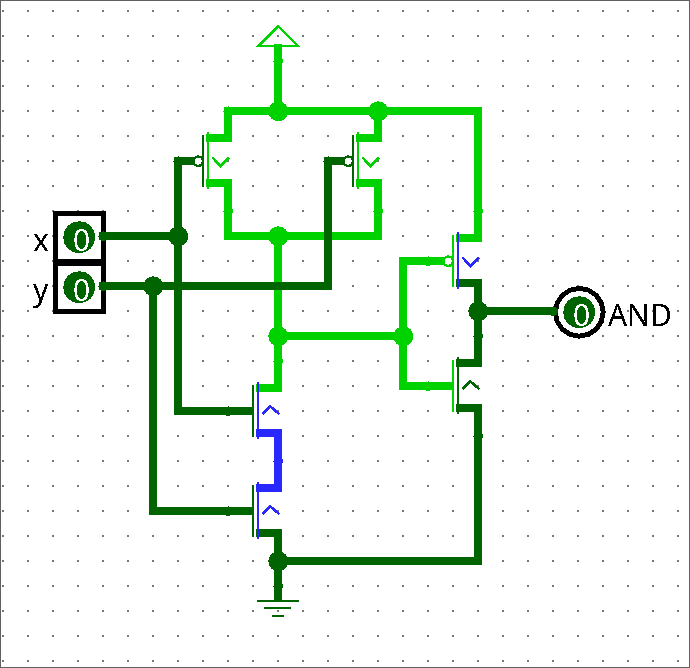
\includegraphics[width=0.3\linewidth]{../images/q1aAND}
		\end{figure}
		מימוש $x + y$: 
		\begin{figure}[H]
			\centering
			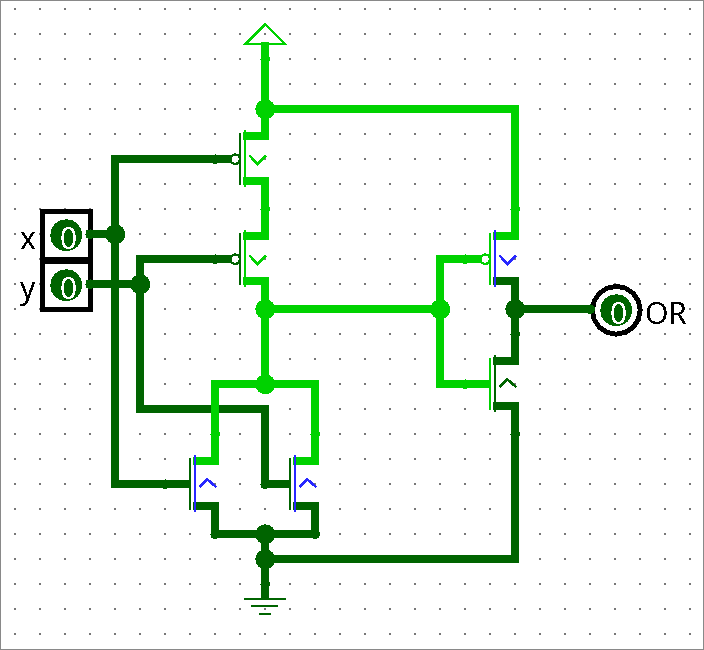
\includegraphics[width=0.3\linewidth]{../images/q1aOR}
			
		\end{figure}
		\item נכתוב את הפונקציה $F$ כפונקציה של $A, B$. 
		\begin{center}
			\begin{tabular}{ c c |c }
					    \en{a} & \en{b} & Out \\
				\hline  0 & 0 & \en{(strong) 0} \\
				\hline  0 & 1 & \en{(strong) 1} \\
				\hline  1 & 0 & \en{(strong) 1} \\
				\hline  1 & 1 & \en{(strong) 1}
			\end{tabular}
		\end{center}
		\item נכתוב את $F$ כפונקציה של $A, B, C$: 
		\begin{center}
			\begin{tabular}{ c c c |c }
				   \en{a} & \en{b} & \en{c} & Out \\
				\hline  0 & 0 & 0 & \en{(strong) 1} \\
				\hline  1 & 0 & 0 & \en{(strong) 1} \\
				\hline  0 & 1 & 0 & \en{(strong) 1} \\
				\hline  1 & 1 & 0 & \en{(strong) 0} \\
				\hline  0 & 0 & 1 & \en{(strong) 0} \\
				\hline  0 & 1 & 1 & \en{(strong) 0} \\
				\hline  1 & 0 & 1 & \en{(strong) 0} \\
				\hline  1 & 1 & 1 & \en{(strong) 0}
			\end{tabular}
		\end{center}
		ולכן: 
		\[ F = a'b'c' + ab'c'  +a'bc' \]
		(אפשר לצמצם עם קרנו במידת הצורך – לא התבקשנו לעשות את זה)
		
	\end{enumerate}
	
	\section{}
	נתונים And, Or, Not. נממש: 
	\begin{enumerate}
		\item מקודד (Encoder) $8 \to 3$: 
		\begin{figure}[H]
			\centering
			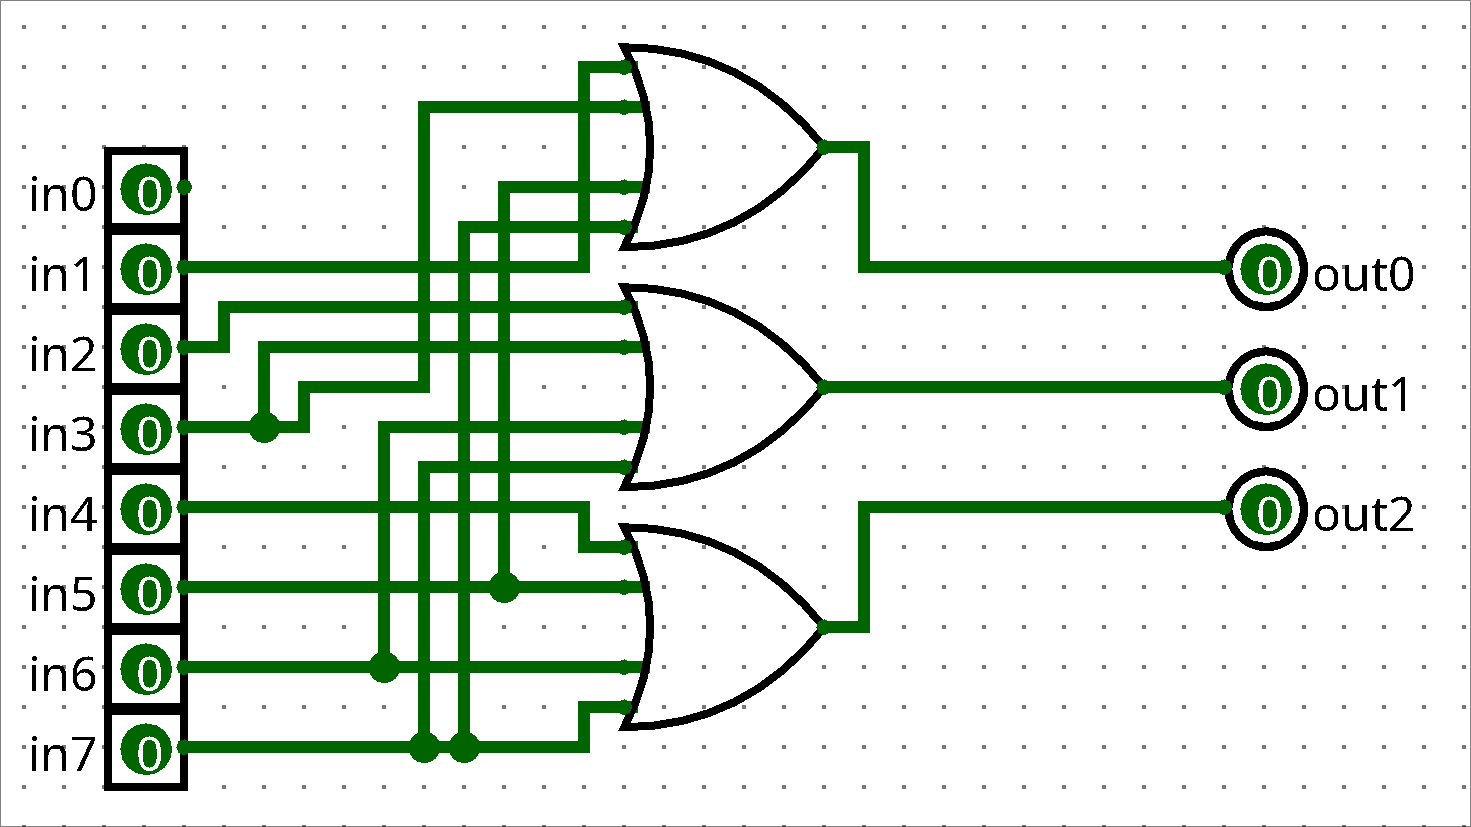
\includegraphics[width=0.4\linewidth]{../images/q2a}
		\end{figure}
		
		
		\item מרבב (MUX) $2 \to 1$: 
		
		\begin{figure}[H]
			\centering
			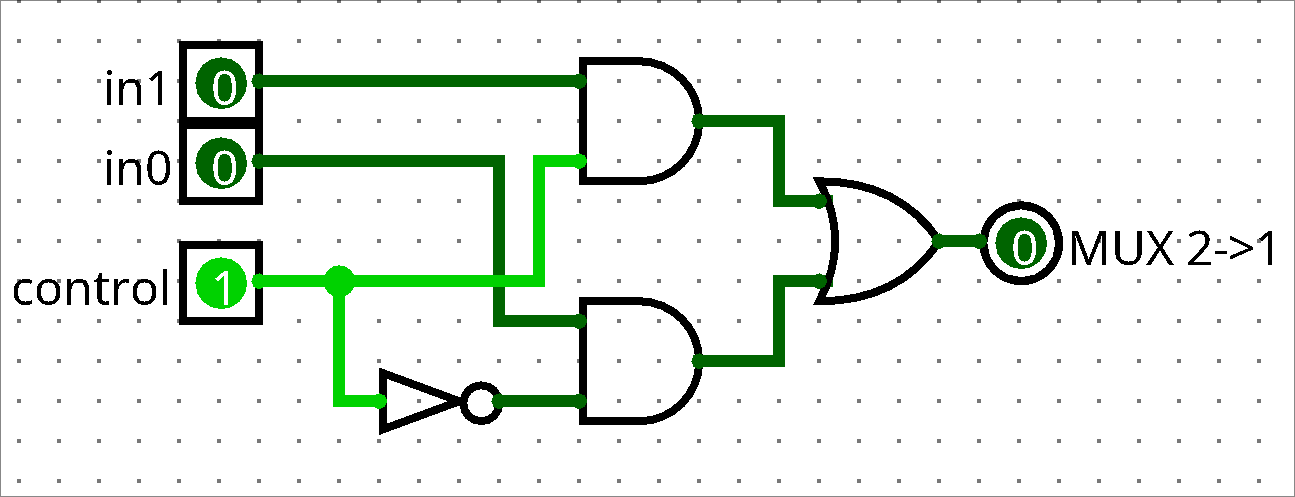
\includegraphics[width=0.4\linewidth]{../images/q2b}
		\end{figure}
		
	\end{enumerate}
	
	\section{}
	\begin{enumerate}[(A)]
		\item נמצא את טווח המספרים בייצוג לש 16 ביטים. 
		
		גודל טווח המספרים הוא $2^{16}$, שמתוכו $\frac{2^{16}}{2} - 1 = 2^{15} - 1$ חיוביים, $\frac{2^{16}}{2}  =   2^{15 } - 1$ שליליים, ואחד מהם הוא $0$. סה''כ הטווח הוא: 
		\[ \csb{-2^{15}, 2^{15} -1} \cap \Z \]
		\item נתבונן במימוש הראשון למחבר מלא:
		\newcommand\cin{\mathrm{C_{in}}}
		\newcommand\cout{\mathrm{C_{out}}}
		\newcommand\s{\mathrm{S}}
		\begin{align*}
			(1) \ \cout = y\cin + x\cin + xy && (1) \ \s = xy' \cin' + x'y'\cin + xy\cin + x'y\cin'
		\end{align*}
		נתבונן במימוש $2$ (כאשר $\otimes$ זה XOR): 
		\begin{align*}
			(2) \ \cout = (xy) + (\cin \cdot (x \otimes y))
			&& (2) \ \s = (x\otimes y)\otimes \cin
		\end{align*}
		נוכיח שקילות לוגית באמצעות אלגברה בוליאנית. 
		\begin{proof}
			ראשית נתחיל מ־$\s$. נבחין ש־$a \otimes b = (ab') + (a'b)$
			\begin{align*}
				(2) \ \s &= (x \otimes y) \otimes \cin = (xy' + x'y) \cin' + \underbrace{(xy' + x'y)'}_{\mathclap{(x' + y)(x + y') = x'y' + xy + \cancel{x'x} + \cancel{yy'}}}\cin \\
				&= xy'\cin' + x'y\cin' + x'y'\cin + xy\cin = (1) \s
			\end{align*}
			כנדרש. אשר ל־$\cout$:
			\[ (2)\ \cout = (xy) + (\cin \cdot (xy' + x'y)) = xy + {xy'\cin + x'y\cin} = xy + y\cin + x\cin = (1) \ \cout \]
		\end{proof}
		\item נממש מעגל המייצג פעולת כפל של מספר בן 2 סיביות למספר בן 3 סיביות: 
		\begin{figure}[H]
			\centering
			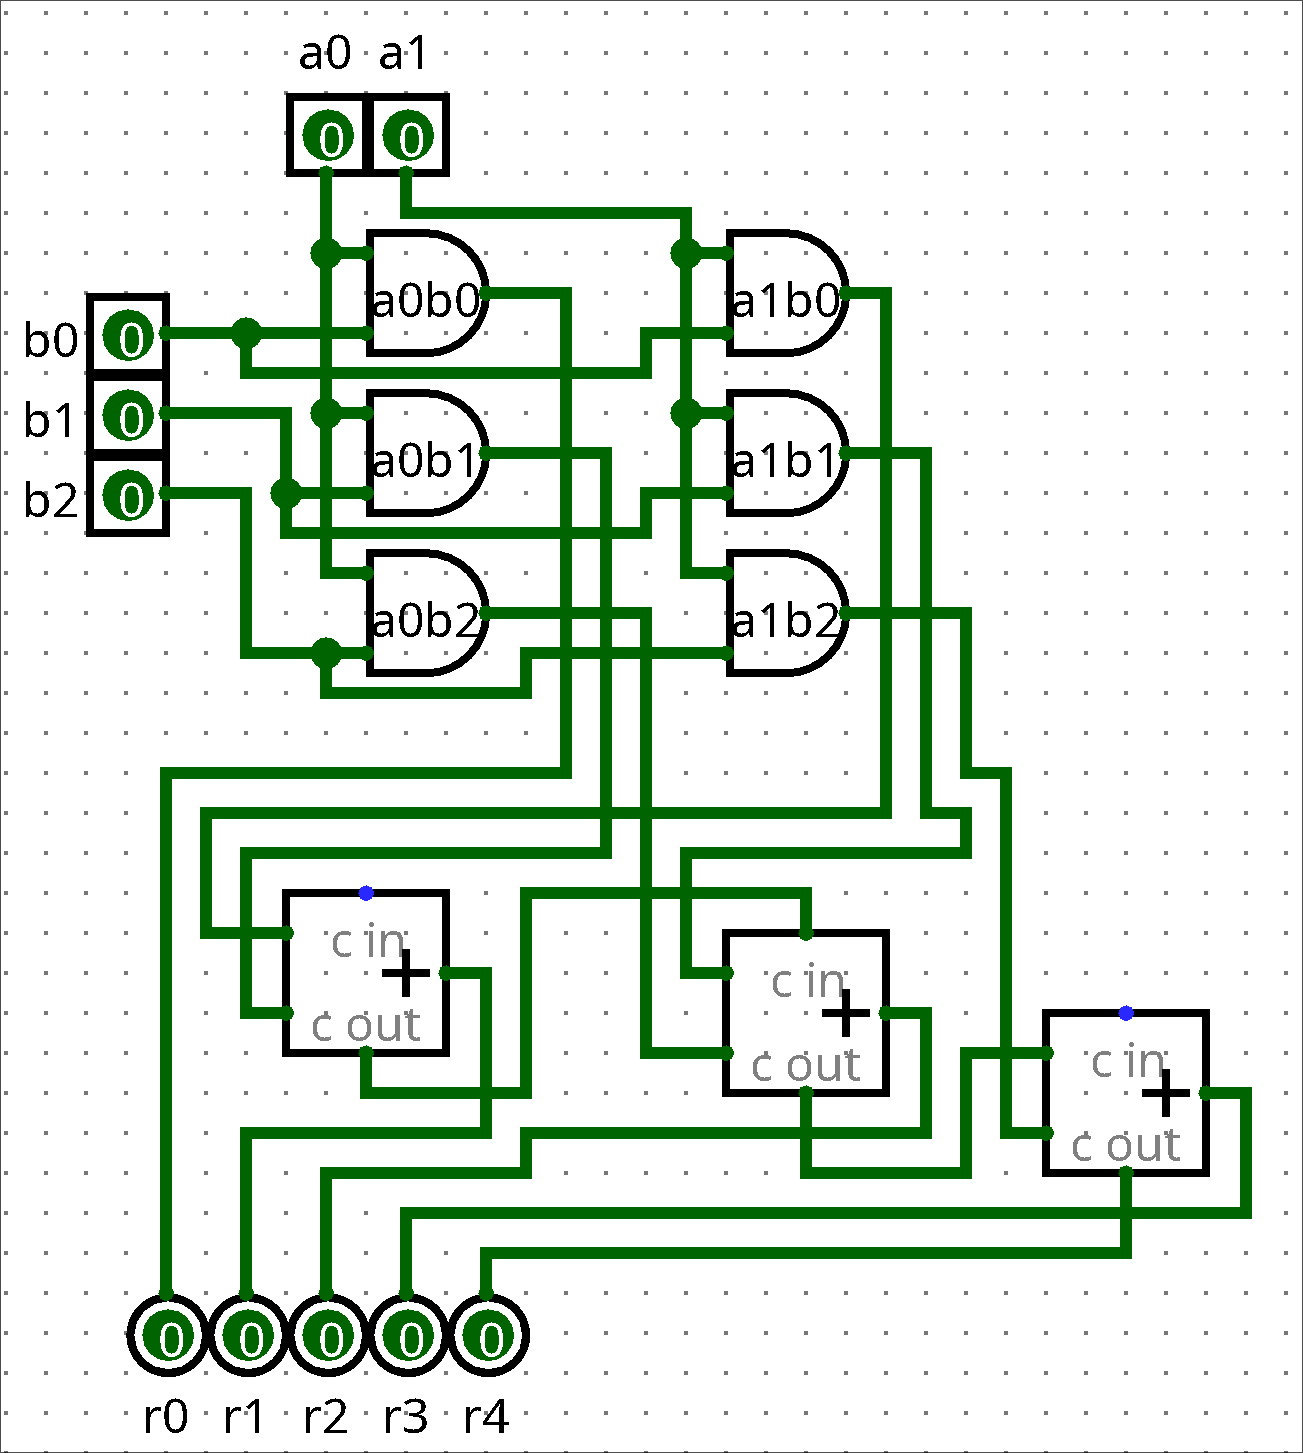
\includegraphics[width=0.4\linewidth]{../images/q3c}
		\end{figure}
		
		\item בעבור שני מספרים בינאריים $A =a_2a_1a_0, B = b_2b_1b_0$ נבנה מעגל שמקבל את $A$ ו־$B$ ומחזיר שלוש סיביות $G, E, L$ כך ש־$L = 1 \iff A < B, E = 1 \iff A = B \land G = 1 \iff A > B$, בלי להשתמש במחסרים. 
		
		\begin{figure}[H]
			\centering
			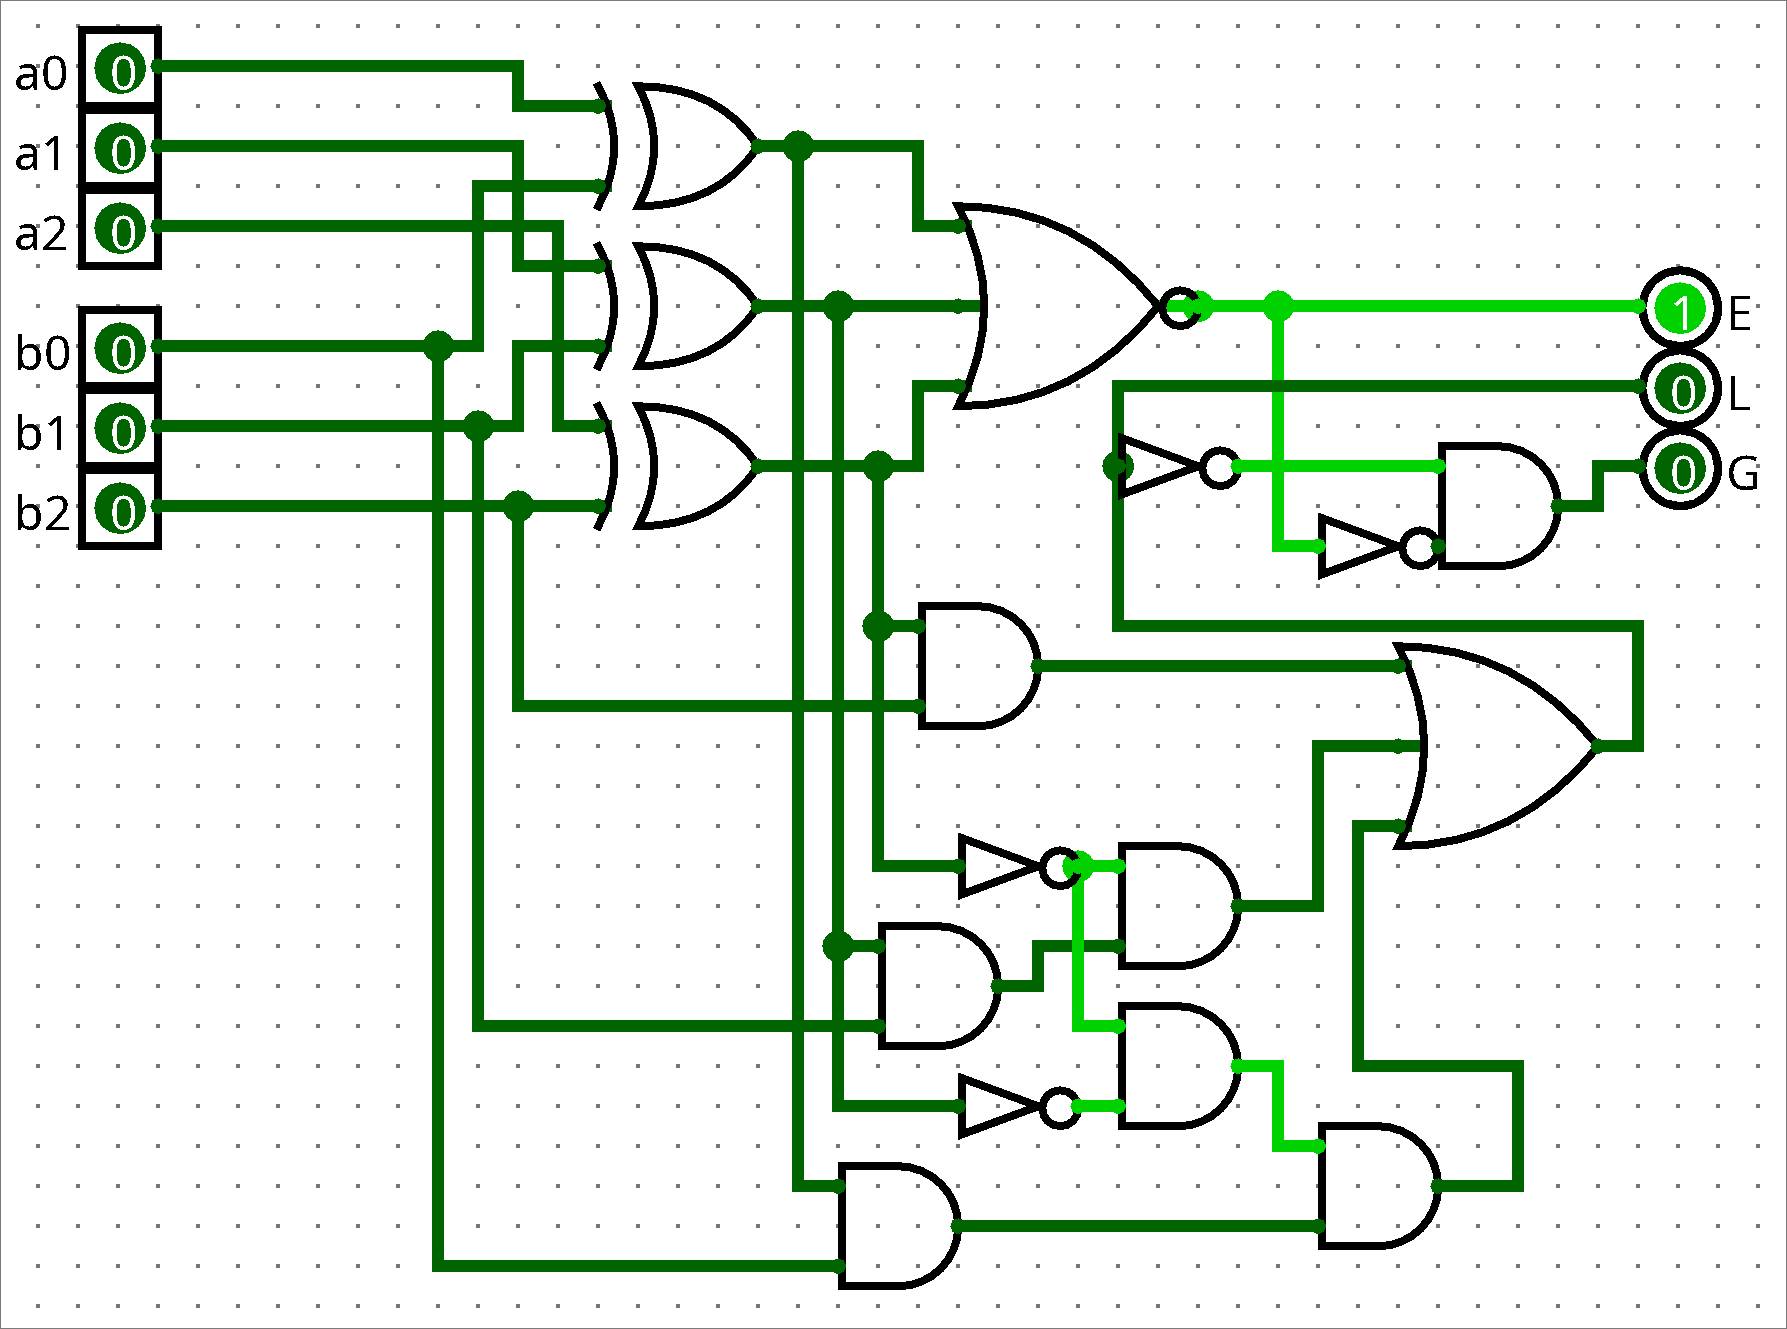
\includegraphics[width=0.4\linewidth]{../images/q3d}
		\end{figure}
		\item מערכת מקבלת קלט בן 4 סיביות ומוציאה $1$ כאשר מספר אחדים בכניסותיו זוגי. נממש אותה באמצעות DeMux $3 \to 8$ ושני שערים לוגיים. 
		
		\begin{figure}[H]
			\centering
			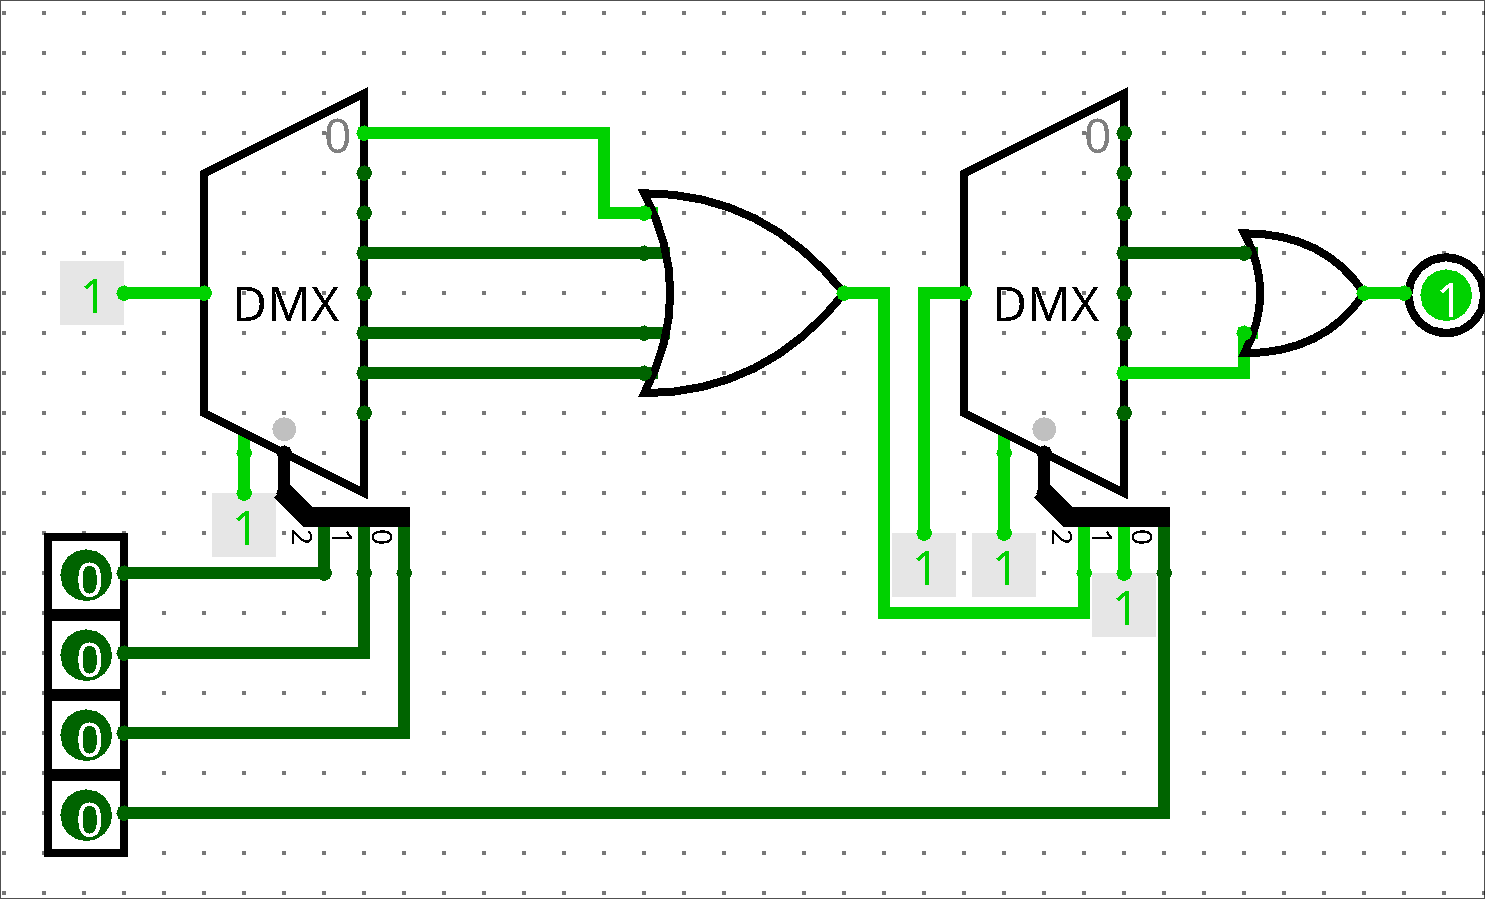
\includegraphics[width=0.4\linewidth]{../images/q3e}
		\end{figure}
		
	\end{enumerate}
	
	\section{}
	נוכיח טענות. 
	\begin{enumerate}[(A)]
		\item ניתן לממש בעזרת MUX $2 \to 1$ ו־$0, 1$ את השער NOT. 
		
		לשם כך, נציג מימוש מפורש: 
		\begin{figure}[H]
			\centering
			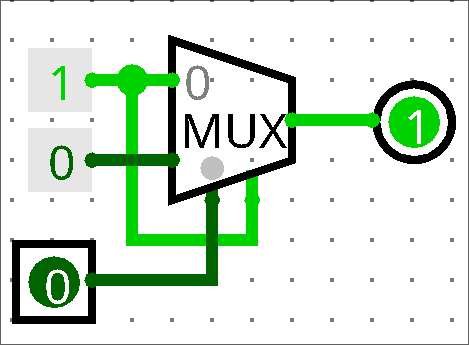
\includegraphics[width=0.2\linewidth]{../images/q4a}
		\end{figure}
		
		\item ניתן לממש באמצעות MUX $2 \to 1$ והקבועים $0, 1$ את השער AND. 
		
		לשם כך, נציב מימוש מפורש: 
		\begin{figure}[H]
			\centering
			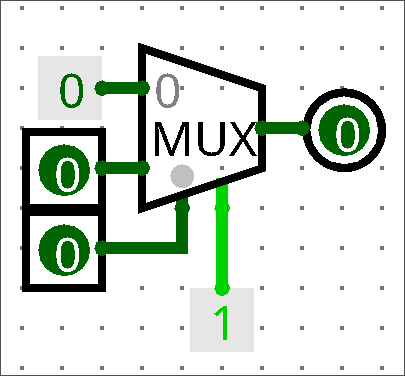
\includegraphics[width=0.2\linewidth]{../images/q4b}
		\end{figure}
	\end{enumerate}
	
	\section{}
	נממש מחסר בשלבים. רוב השאלה ב־logisim. 
	\begin{enumerate}[(A)]
		\item נממש חצי מחסר עם כניסות $x,y, \mathrm D, \mathrm{B_{out}}$. 
		\begin{enumerate}
			\item ראשית, נמצא את טבלת האמת: 
			\begin{center}
				\begin{tabular}{ c c | c c}
					\en{x} & \en{y} & $\mathrm D$ & $\mathrm{B_{out}}$ \\
					\hline  0 & 0 & 0 & 0 \\
					\hline  0 & 1 & 1 & 1 \\
					\hline  1 & 0 & 1 & 0 \\
					\hline  1 & 1 & 0 & 0
				\end{tabular}
			\end{center}
			\item תמונה של המימוש ב־logisim: 
			\begin{figure}[H]
				\centering
				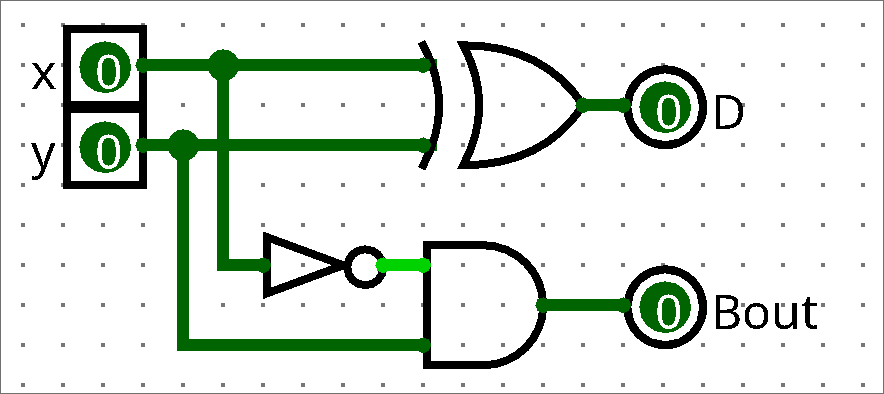
\includegraphics[width=0.3\linewidth]{../images/q5a}
			\end{figure}
		\end{enumerate}
		\item נממש מחסר מלא באמצעות שני חצאי מחסר ושער לוגי. תמונה של המימוש ב־logisim: 
		\begin{figure}[H]
			\centering
			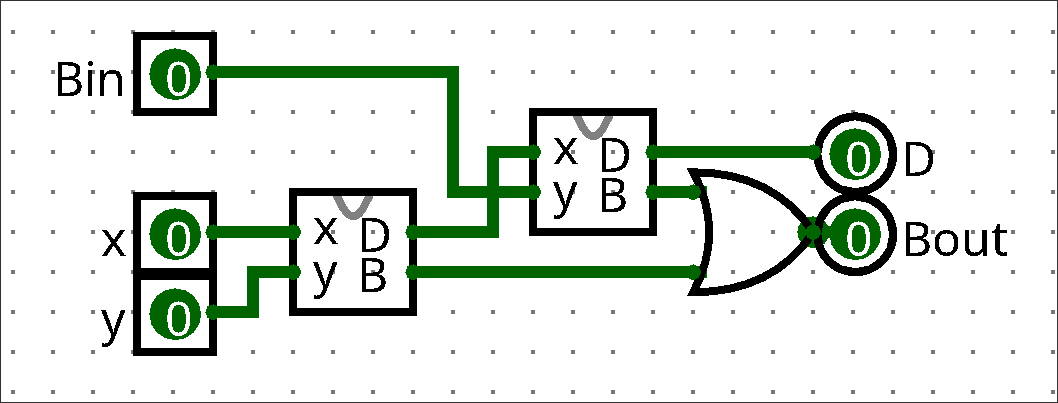
\includegraphics[width=0.3\linewidth]{../images/q5b}
		\end{figure}
		\item נממש מחסר מלא בעזרת מחבר מלא. תמונה של המימוש ב־logisim: 
		\begin{figure}[H]
			\centering
			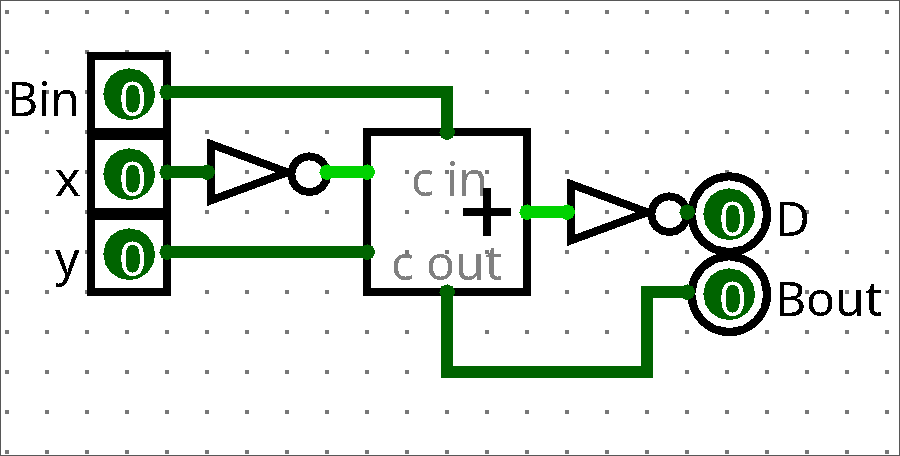
\includegraphics[width=0.3\linewidth]{../images/q5c}
		\end{figure}
	\end{enumerate}
	
	
	\ndoc
\end{document}
